\subsection{Архитектура решения}

Общая схема решения представлена на рис. \ref{fig:solution_overview}.

\begin{figure}[h!]
    \centering
    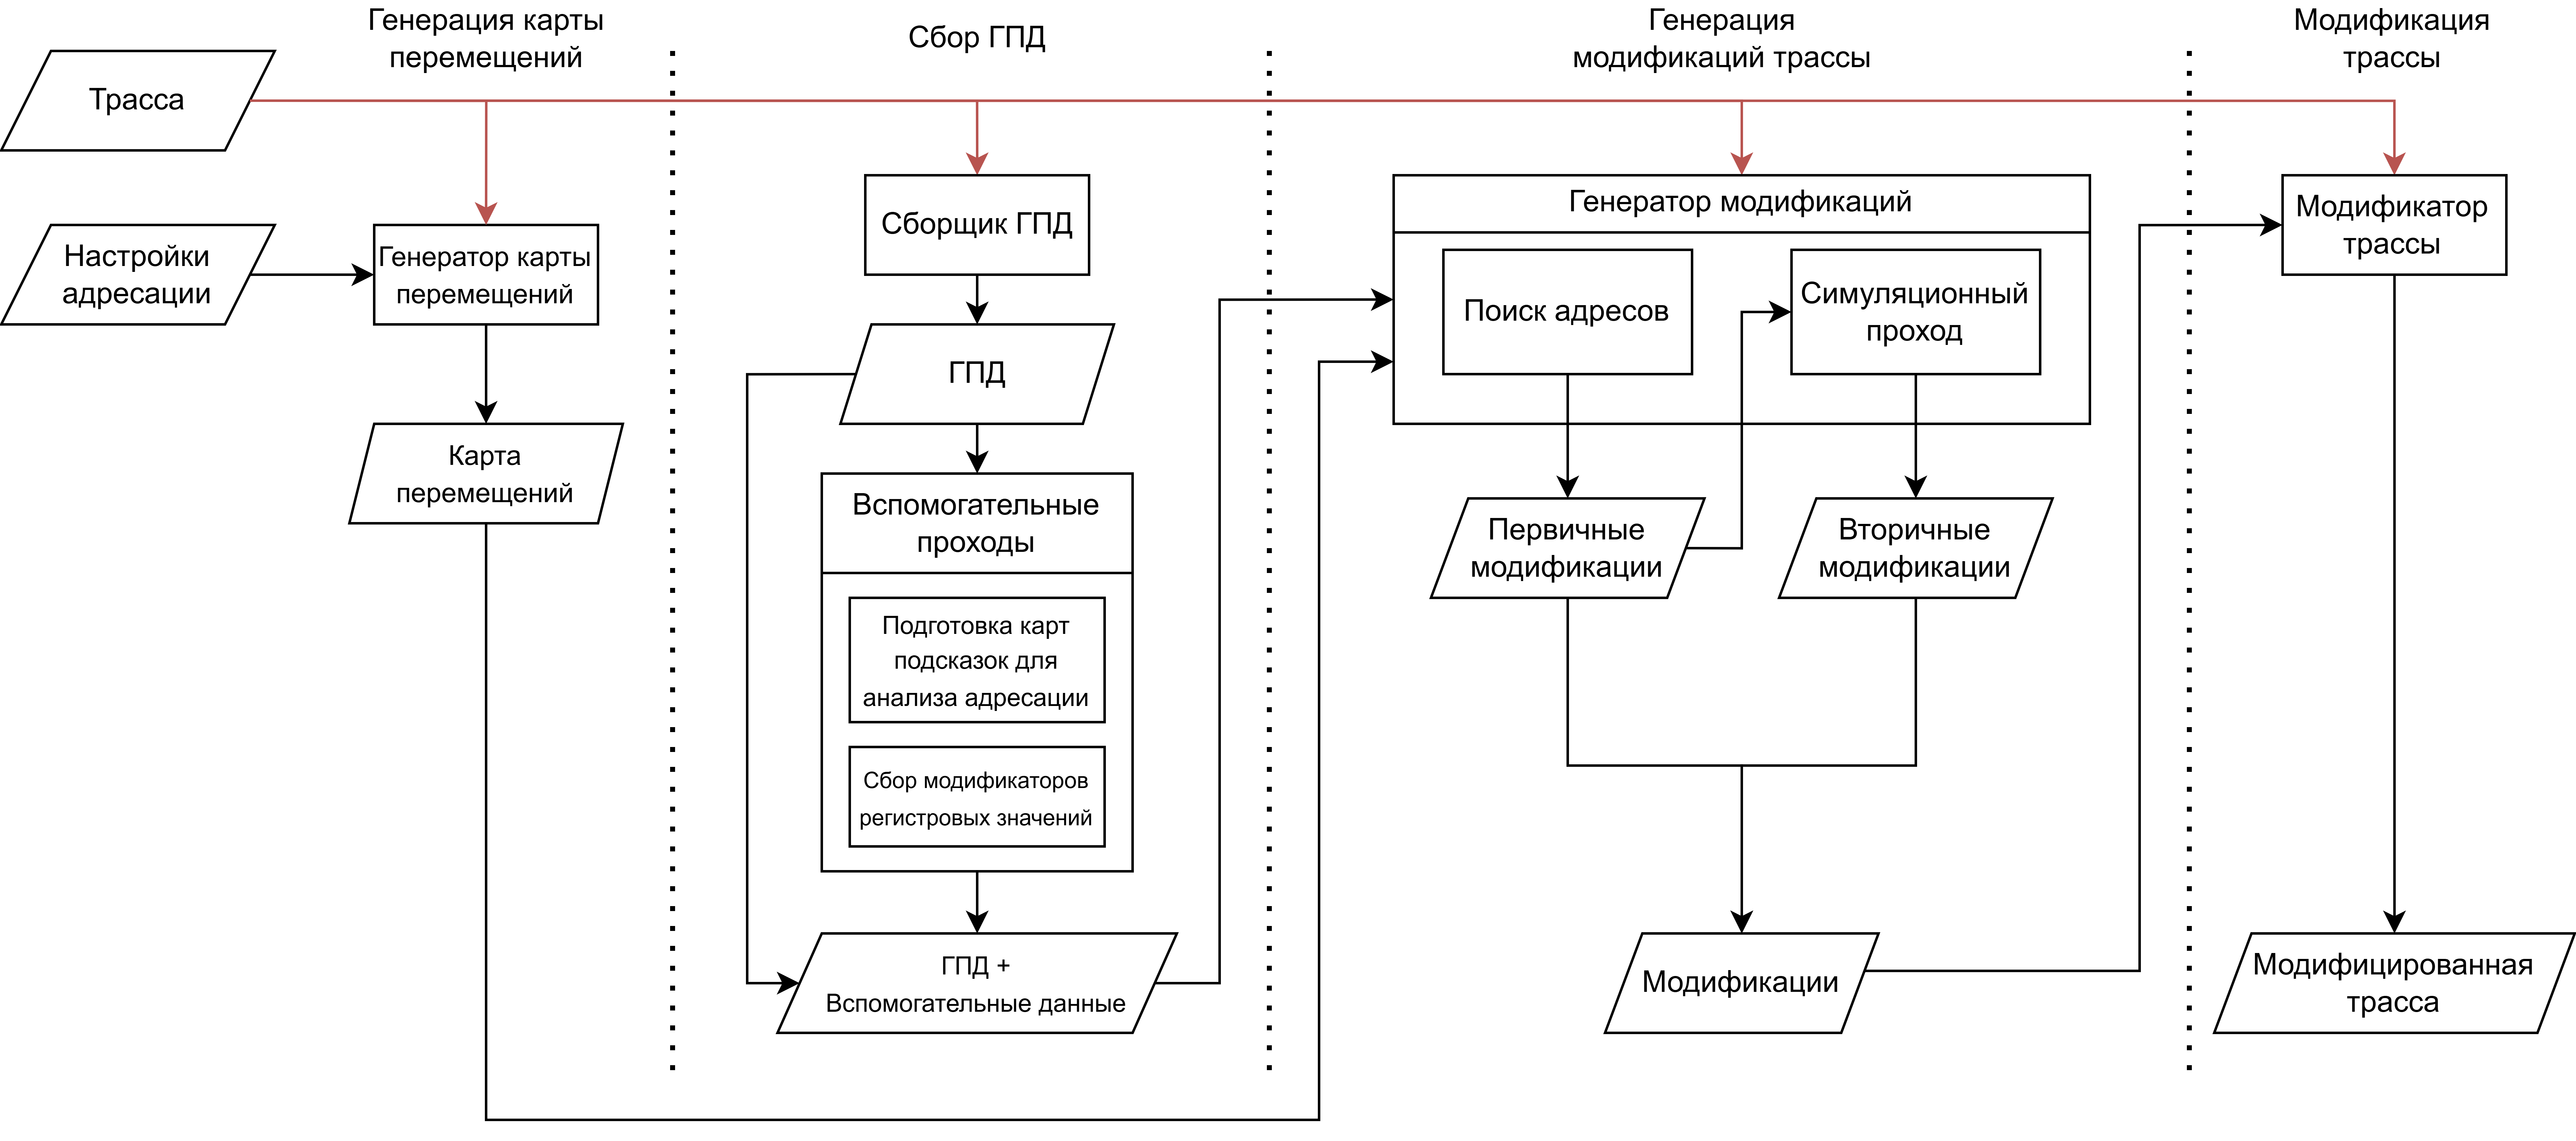
\includegraphics[width=\linewidth]{pics/solution_overview.drawio.png}
    \caption{Общая схема решения.}
    \label{fig:solution_overview}
\end{figure}
\FloatBarrier

Обработка трассы происходит в четыре стадии:

\begin{enumerate}
    \item Генерация карты перемещений

    На этой стадии генерируется карта перемещений областей памяти, удовлетворяющая новым ограничениям, обусловленным изменением настроек адресации.

    \item Сбор графа потока данных (\gls{dfg})

    На данной стадии осуществляется симуляционный проход по трассе, в ходе которого собирается ГПД. Затем осуществляется ряд обходов графа, в ходе которых собирается вспомогательная информация, размечающая его.

    \item Генерация модификаций трассы

    Генерация происходит в два этапа:

    \begin{enumerate}
        \item Поиск адресов на ГПД и генерация первичных модификаций

        \item Симуляционный проход по модифицированной трассе и генерация вторичных модификаций
    \end{enumerate}

    \item Запись модифицированной трассы
\end{enumerate}

Генерируемые модификации могут изменять существующие и добавлять новые записи, обеспечивая консистентность выходной трассы. Примеры возможных модификаций были представлены в разделе \ref{sec:execution_traces}. Некоторые модификации могут снижать репрезентативность выходной трассы, так как будут приводить к изменению целевых счетчиков при дальнейшей ее обработке.
